\chapter{DESIGN}
\section{Introduction}
%write about project design
The design of SecureEdgeNet follows a modular machine learning systems architecture. The project separates concerns into data preparation, federated client training, server aggregation, model definitions, ensemble prediction, evaluation, checkpointing, and inference. This separation makes the system easier to test, extend, and explain. The key design decision is to use Federated Learning for models whose parameters can be numerically averaged, while handling XGBoost as a client-local ensemble component. Logistic Regression and MLP models expose continuous parameters such as coefficients, intercepts, weight matrices, and bias vectors. These can be aggregated using FedAvg. XGBoost, however, consists of tree structures, split thresholds, and leaf nodes. These structures cannot be meaningfully averaged using simple FedAvg. Therefore, XGBoost improves the final system through probability-level ensembling.

Additionally, the architecture is designed to simulate real-world banking environments where data remains decentralized across multiple institutions. Each federated client independently preprocesses and trains on its own transaction partition, ensuring that raw financial records never leave the local environment. The ensemble layer combines the strengths of linear, nonlinear, and tree-based learning methods to improve robustness against diverse fraud patterns. The system also emphasizes scalability and reproducibility by using modular configuration-driven pipelines that can be extended to additional clients or models with minimal architectural changes. By integrating privacy-preserving distributed learning with ensemble intelligence, the platform balances detection accuracy, interpretability, and practical deployment feasibility for modern fraud detection systems.

\section{Architecture Design}
% as per the selected architectural style (Structure diagram (structured approach) or class diagram (Object oriented approach)
%explain all the diagrams
\begin{figure}[H]
\centering
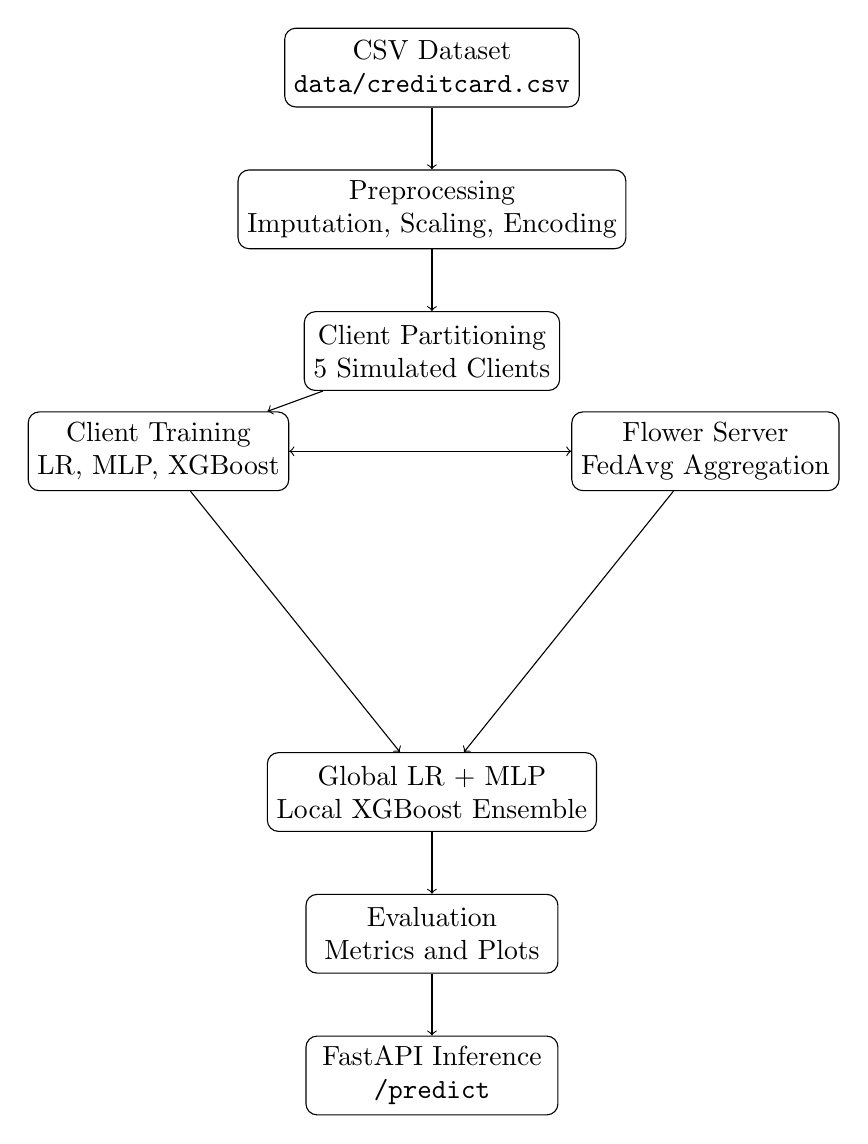
\begin{tikzpicture}[node distance=1.8cm, every node/.style={draw, rounded corners, align=center, minimum width=3.2cm, minimum height=1cm}]
\node (data) {CSV Dataset\\\texttt{data/creditcard.csv}};
\node (prep) [below of=data] {Preprocessing\\Imputation, Scaling, Encoding};
\node (part) [below of=prep] {Client Partitioning\\5 Simulated Clients};
\node (client) [below left of=part, xshift=-2.2cm] {Client Training\\LR, MLP, XGBoost};
\node (server) [below right of=part, xshift=2.2cm] {Flower Server\\FedAvg Aggregation};
\node (global) [below of=part, yshift=-3.8cm] {Global LR + MLP\\Local XGBoost Ensemble};
\node (eval) [below of=global] {Evaluation\\Metrics and Plots};
\node (api) [below of=eval] {FastAPI Inference\\\texttt{/predict}};
\draw[->] (data) -- (prep);
\draw[->] (prep) -- (part);
\draw[->] (part) -- (client);
\draw[->] (client) -- (server);
\draw[->] (server) -- (client);
\draw[->] (server) -- (global);
\draw[->] (client) -- (global);
\draw[->] (global) -- (eval);
\draw[->] (eval) -- (api);
\end{tikzpicture}
\caption{System Architecture of SecureEdgeNet}
\label{fig:architecture}
\end{figure}

Figure \ref{fig:architecture} shows the complete architecture. The dataset is loaded and preprocessed centrally for simulation, then partitioned into clients. During training, each client uses only its own local partition. The Flower server aggregates Logistic Regression and MLP parameters. XGBoost models remain client-local and contribute to the final ensemble through their predicted probabilities.

\subsection{Federated Aggregation Design}
For a client $k$ with $n_k$ samples and locally trained parameters $W_k$, FedAvg computes:
\begin{equation}
W_{global} = \frac{\sum_{k=1}^{K} n_k W_k}{\sum_{k=1}^{K} n_k}
\end{equation}
This weighting prevents a small client and a large client from having equal influence when their sample counts differ.

\subsection{Ensemble Design}
The final fraud score is:
\begin{equation}
s_{final} = 0.3s_{LR} + 0.3s_{MLP} + 0.4s_{XGB}
\end{equation}
where $s_{XGB}$ is the average probability from all client-local XGBoost models.

\section{User Interface Design}
% explain all the diagrams
The project does not implement a graphical user interface. The user interacts with the system through command-line scripts, notebook cells, generated plots, saved checkpoints, and the FastAPI inference endpoint. This design is suitable for research and Google Colab environments.

The inference API accepts transaction features and returns:
\begin{itemize}
    \item fraud probability,
    \item fraud decision,
    \item threshold,
    \item model confidence,
    \item model contribution scores.
\end{itemize}

Example request format:
\begin{lstlisting}[language=Python, caption={Example API Payload}]
{
    "features": {
        "Time": 0,
        "V1": -1.3598,
        "V2": -0.0727,
        "Amount": 149.62
    }
}
\end{lstlisting}

\section{State Diagram}
%(Flowchart (structured approach) or Sequence and state diagram (Object oriented approach))
%explain all the diagrams
\begin{figure}[H]
\centering
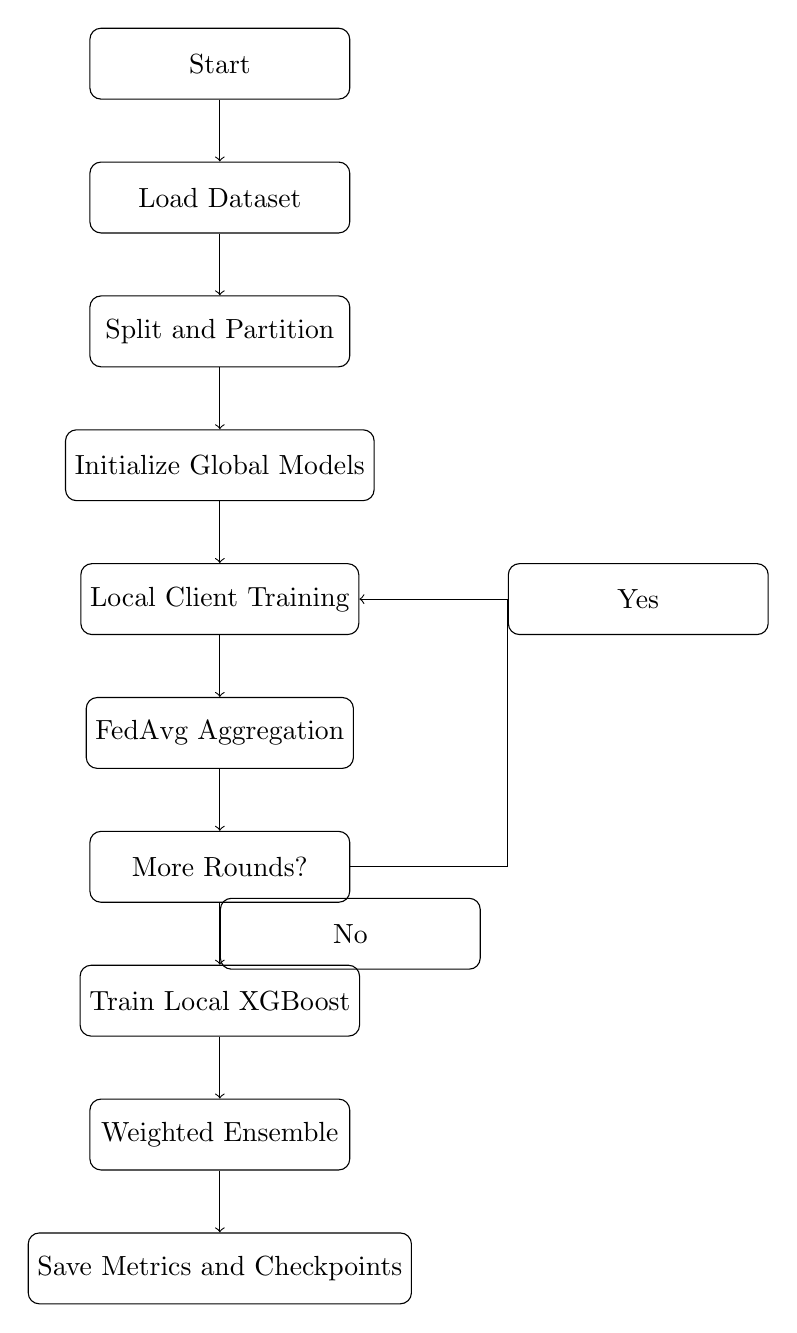
\begin{tikzpicture}[node distance=1.7cm, every node/.style={draw, rounded corners, align=center, minimum width=3.3cm, minimum height=0.9cm}]
\node (start) {Start};
\node (load) [below of=start] {Load Dataset};
\node (split) [below of=load] {Split and Partition};
\node (init) [below of=split] {Initialize Global Models};
\node (local) [below of=init] {Local Client Training};
\node (agg) [below of=local] {FedAvg Aggregation};
\node (round) [below of=agg] {More Rounds?};
\node (xgb) [below of=round] {Train Local XGBoost};
\node (ens) [below of=xgb] {Weighted Ensemble};
\node (save) [below of=ens] {Save Metrics and Checkpoints};
\draw[->] (start) -- (load);
\draw[->] (load) -- (split);
\draw[->] (split) -- (init);
\draw[->] (init) -- (local);
\draw[->] (local) -- (agg);
\draw[->] (agg) -- (round);
\draw[->] (round.east) -- ++(2,0) |- node[right]{Yes} (local.east);
\draw[->] (round) -- node[right]{No} (xgb);
\draw[->] (xgb) -- (ens);
\draw[->] (ens) -- (save);
\end{tikzpicture}
\caption{Training State Flow}
\label{fig:training_state}
\end{figure}

Figure \ref{fig:training_state} describes the training state flow. The system repeats local training and aggregation for the configured number of federated rounds. After federated rounds finish, the XGBoost models are trained locally and the final ensemble is evaluated.
